%%%%%%%%%%%%%%%%%%%%%%%%%%%%%%%%%%%%%%%%%
% Journal Article
% LaTeX Template
% Version 2.0 (February 7, 2023)
%
% This template originates from:
% https://www.LaTeXTemplates.com
%
% Author:
% Vel (vel@latextemplates.com)
%
% License:
% CC BY-NC-SA 4.0 (https://creativecommons.org/licenses/by-nc-sa/4.0/)
%
% NOTE: The bibliography needs to be compiled using the biber engine.
%
%%%%%%%%%%%%%%%%%%%%%%%%%%%%%%%%%%%%%%%%%

%----------------------------------------------------------------------------------------
%	PACKAGES AND OTHER DOCUMENT CONFIGURATIONS
%----------------------------------------------------------------------------------------

\documentclass[
	a4paper, % Paper size, use either a4paper or letterpaper
	10pt, % Default font size, can also use 11pt or 12pt, although this is not recommended
	% unnumberedsections, % Comment to enable section numbering
	twoside, % Two side traditional mode where headers and footers change between odd and even pages, comment this option to make them fixed
]{LTJournalArticle}

\usepackage{
	amsmath,
	tikz,
}

\usetikzlibrary{shapes.geometric, shapes.symbols, arrows, positioning, calc, fit, backgrounds}
\input{flowchart_defs.tex}

\DeclareMathOperator*{\argmin}{\arg\!\min}
\DeclareMathOperator*{\argmax}{\arg\!\max}

\addbibresource{bibliography.bib} % BibLaTeX bibliography file

\runninghead{Piranha Plants as Charade} % A shortened article title to appear in the running head, leave this command empty for no running head

% \footertext{\textit{Journal of Biological Sampling} (2024) 12:533-684} % Text to appear in the footer, leave this command empty for no footer text

\setcounter{page}{1} % The page number of the first page, set this to a higher number if the article is to be part of an issue or larger work

%----------------------------------------------------------------------------------------
%	TITLE SECTION
%----------------------------------------------------------------------------------------

\title{Piranha Plants as Charade: Exploring \\ Melody-Guided, Algorithmic Music Generation} % Article title, use manual lines breaks (\\) to beautify the layout

% Authors are listed in a comma-separated list with superscript numbers indicating affiliations
% \thanks{} is used for any text that should be placed in a footnote on the first page, such as the corresponding author's email, journal acceptance dates, a copyright/license notice, keywords, etc
\author{Max Huang, Emily Yu}
% \author{%
% 	John Smith\textsuperscript{1,2}, Robert Smith\textsuperscript{3} and Jane Smith\textsuperscript{1}\thanks{Corresponding author: \href{mailto:jane@smith.com}{jane@smith.com}\\ \textbf{Received:} October 20, 2023, \textbf{Published:} December 14, 2023}
% }

% Affiliations are output in the \date{} command
\date{April 4, 2025}
% \date{\footnotesize\textsuperscript{\textbf{1}}School of Chemistry, The University of Michigan\\ \textsuperscript{\textbf{2}}Physics Department, The University of Wisconsin\\ \textsuperscript{\textbf{3}}Biological Sciences Department, The University of Minnesota}

\renewcommand{\maketitlehookd}{%
	\begin{abstract}
		\noindent
        The premise of ``Piranha Plants as Charade'' is to transform a melody into a full-fledged song in the style of ``Piranha Plants on Parade'' from the video game ``Super Mario Bros. Wonder''. Given an input melody in the form of a digital signal (e.g. a WAV file), we developed a music generation algorithm that transforms the input with the following process: 1) it extracts the melodic information from the input; 2) it generates a chord progression that fits under both the extracted melody and the appropriate stylistic conventions; 3) it generates a musical accompaniment based on the melody and chord progression; and 4) it exports the generated accompaniment as a WAV file. For inputs within the targeted scope (i.e. in 4/4, in C major, and at 110 BPM), our algorithm can often produce convincing results, but for a majority of the cases, the output is subpar. Step 1 (melody extraction) is most likely the largest source of failure; the pitch detection is generally correct, however, the onset detection often produces false positives. Despite the current shortcomings, we believe that the core ideas behind ``Piranha Plants as Charade'' can be extended upon to adequately meet the premise we set. We plan on fine-tuning our algorithm and further iterating over our code to produce better results.
	\end{abstract}
}

%----------------------------------------------------------------------------------------

\begin{document}

\maketitle % Output the title section

%----------------------------------------------------------------------------------------
%	ARTICLE CONTENTS
%----------------------------------------------------------------------------------------

\section{Introduction}

The fields of mathematics and music are heavily intertwined. In the late 16th-century, many Western European music theorists believed that they had developed \emph{ars perfecta}: a set of rules for which, if followed, guaranteed that music be ``free of reprehensible elements, purged of every error and polished, and [the] harmonies will be good and pleasant'' \autocite{Richard:2005}. Although the concept of \emph{ars perfecta} is irrelevant in modern times, we sympathize with their aspirations to model musical correctness with rule-based approaches. We wanted to explore the relationship between music and mathematics in a similar manner by generating music using rule-based algorithms that humans follow --- processes that mirror the human composer. Our goal was to create a computer program that transforms a melody into a full-fledged song in the style of ``Piranha Plants on Parade'', a song from the video game \emph{Super Mario Bros. Wonder}.

We believe that ``Piranha Plants on Parade'' was an apt song to emulate for our proof-of-concept. It is based on a relatively simple harmonic framework, which lets us focus on developing the algorithm's high-level concepts rather than on hard-coding harmonic rules; yet the transitions between harmonic states\footnote{The chord changes.} are distinct enough to be recognizable. Similarly, the song's accompaniment\footnote{The music besides the melody.} style is repetitive enough such that it can be approximated with only a few rules. ``Piranha Plants on Parade'' also distinctively features gibberish lyrics, which lets us explore vocal generation without worrying about conforming to an existing language. Lastly, the song originates from a video game, a medium with a history of synthetic music, thus we believe it to be a thematically appropriate subject for computer generated music.


\section{System Overview}

Given an input melody in the form of a digital signal, we developed a music generation algorithm that transforms the input with these steps: 1) extract the melodic information from the input; 2) generate a chord progression that fits under both the extracted melody and the appropriate stylistic conventions; 3) generate a musical accompaniment based on the melody and chord progression; and 4) export the generated accompaniment as a WAV file (see Figure \ref{fig:architecture}).

\subsection{Melody Extraction}
\label{sec:melody_extraction}

The first step in Piranha Plants as Charade is to extract the melody from the input audio. The goal of this section is to take an audio file and output a sequence of notes, each with a MIDI pitch, start time, and duration. This problem can be broken down into two subproblems: pitch detection and note segmentation.

As a pre-processing step, we first apply the Harmonic-Percussive Source Separation (HPSS) algorithm \autocite{HPSS:2010,HPSS:2014} to separate the harmonic and percussive components of the audio signal. We perform pitch detection on the harmonic component and use the percussive component to identify the timestamps where notes start, which we refer to as note onsets. Finally, we combine both components to produce the final sequence of notes.

\subsubsection{Pitch Detection}

This problem determines the fundamental frequency of a sound; we aim to produce a sequence of MIDI pitches that correspond to notes in the melody. We explored a few different approaches, starting with cepstrum analysis and autocorrelation. However, these methods failed to handle the complexity of imperfect audio. We elaborate more upon this in Section \ref{sec:avenues}. We decided to use the PYIN algorithm as implemented in the librosa library, which is a state-of-the-art pitch detection algorithm that builds upon autocorrelation to detect pitches more robustly.

The PYIN algorithm \autocite{PYIN:2014} is robust on imperfect audio and has a readily available implementation in the librosa library\footnote{\href{https://librosa.org/doc/0.11.0/generated/librosa.pyin.html}{librosa.org/doc/0.11.0/generated/librosa.pyin.html}}, which allowed us to focus on the higher-level aspects of our project. PYIN is a state-of-the-art pitch detection algorithm that builds upon autocorrelation to handle audio more robustly. At a high level, PYIN applies autocorrelation to detect pitch candidates and refines the result using a probabilistic thresholding model to filter out spurious frequencies.

After applying PYIN to the harmonic component of the audio signal, we have the estimated pitch in hertz across time. We then apply multiple pitch shifts by a few cents \footnote{A logarithmic unit representing a hundredth of a semitone.} to find the best match, determined by the lowest error after rounding to the nearest MIDI pitch.

\subsubsection{Note Segmentation}

Once we have the pitch sequence, it must be segmented into individual notes. To do this, we count quantized time units from the start of the first identified pitch at the assumed tempo of the song. Within each interval, we take the mode of the pitches as the pitch at that time. We end the previous note and begin a new one if either of the following conditions are met:
\begin{enumerate}
    \item The pitch changes from the previous interval.
    \item An onset is detected in the percussive component of the audio at the corresponding time.
\end{enumerate}
Thus, we obtain a sequence of notes defining the melody to pass to the next component.


\subsection{Chord Generation}
\label{sec:chord_generation}

After extracting the melody, the next step in Piranha Plants as Charade is to generate chords that harmonize with the melody. The problem of selecting chords that ``sound good'' with a melody is generally quite open-ended and subjective. For any given melody, there are many different sequences of chords that could harmonize with it, evoking different emotions and styles.To narrow down the scope, our MVP implementation focuses on generating chords adhering with the style of Piranha Plants.

The chord generation component produces a sequence of chords, each defined by a root note and a chord quality. For example, a C major chord has a root note of C and a chord quality of major. In order to determine the ``best'' sequence, we model this problem using the Hidden Markov Model (HMM) framework.

The Hidden Markov Model \autocite{HMM:2023}, depicted in Figure \ref{fig:hmm}, is a statistical model that describes a sequence of hidden states, each of which emits an observation. In the context of chord generation, we model the hidden states as the sequence of chords and the observations as a function of the melody. The HMM framework allows us to model the probability of a chord sequence given a melody, which we can then use to generate the most likely or most favorable sequence of chords.

The model consists of the following components for time step $t \geq 0$:
\begin{itemize}
    \item \textbf{States} $s_t$: The hidden states of the model, which represent the sequence of chords.
    \item \textbf{Observations} $o_t$: The observations of the model, which represent the melody.
    \item \textbf{Initial State Probabilities (Priors)} $P(s_0)$: The probabilities of starting in a particular state.
    \item \textbf{Transition Probabilities} $P(s_{t+1} | s_t)$: The probabilities of transitioning between states.
    \item \textbf{Observation Probabilities} $P(o_t | s_t)$: The probabilities of emitting an observation given a state.
\end{itemize}

\begin{figure}
    \centering
    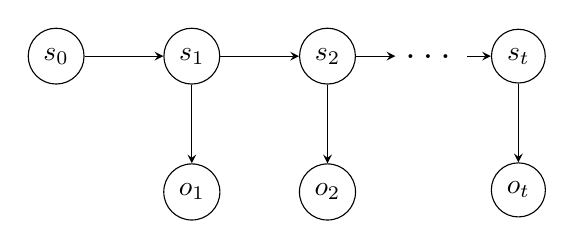
\begin{tikzpicture}[->, >=stealth, node distance=1cm, auto, scale=1, transform shape]
        % Hidden states
        \node[draw, circle] (s0) {$s_0$};
        \node[draw, circle, right=of s0] (s1) {$s_1$};
        \node[draw, circle, right=of s1] (s2) {$s_2$};
        \node[right=0.5cm of s2] (dots) {\Large $\dots$};
        \node[draw, circle, right=0.3cm of dots] (st) {$s_t$};
        
        % Observation states
        \node[draw, circle, below=of s1] (o1) {$o_1$};
        \node[draw, circle, below=of s2] (o2) {$o_2$};
        \node[draw, circle, below=of st] (ot) {$o_t$};
        
        % Hidden state transitions
        \draw[->] (s0) -- (s1);
        \draw[->] (s1) -- (s2);
        \draw[->] (s2) -- (dots);
        \draw[->] (dots) -- (st);
        
        % Observation emissions
        \draw[->] (s1) -- (o1);
        \draw[->] (s2) -- (o2);
        \draw[->] (st) -- (ot);
    \end{tikzpicture}
    \caption{Hidden Markov Model for chord generation.}
    \label{fig:hmm}
\end{figure}

In the most basic case, states and observations can be mapped to integer indices such that the transition and observation probabilities can be represented as matrices. The model can then be solved using the Viterbi algorithm, which is a dynamic programming algorithm that finds the most likely sequence of hidden states given the observations.

For this project, we found it easier to implement the transition and observation probabilities as scores instead to better capture the subjective process of selecting chords. The transition scores represent the favorability of transitioning between two chords, while the observation scores represent the favorability of a chord given the melody.

\subsubsection{Transition Scores}

To define the transitions, we started by restricting the valid states to only a small set of chords that appear in ``Piranha Plants on Parade'': I, IV, and V of the key; and their respective V7 chords. Thus, each of these chords can transition to each other with a constant score.

Another rule we implemented is that the V7 chord must resolve to the I chord. This is a common resolution in music theory, and it is used in ``Piranha Plants on Parade''. We assigned a higher score to this transition to ensure that the model would favor this resolution.

\subsubsection{Observation Scores}

The observation scores are based on the melody. We calculate the score of a melody given a chord by summing the number of notes in the melody that are in the chord. This is a simple heuristic that favors chords that contain more notes from the melody, which is generally a good rule of thumb for harmonization. Although this doesn't fully account for deviations such as passing tones, it provides a good starting point for the model.


\subsection{Accompaniment Generation}

[accompaniment generation]


\subsection{Audio Export}
\label{sec:audio_export}

The final phase of Piranha Plants as Charade is to export the generated song from Part \ref{sec:accompaniment_generation} as a WAV file, a standard audio format. This step is comprised of two independent parts: 1) a pipeline that uses custom samples to handle the vocal parts; and 2) a pipeline that leverages the MIDI standard to handle all other instruments. The two results are added component-wise to generate the overall output.

\subsubsection{MIDI-Based Pipeline}

By building around the MIDI standard, the bulk of this step is handled by external programs. First, the appropriate song data is written to a MIDI file using MIDIUtil, a Python library. Next, the generated file is converted into a WAV file using FluidSynth, an open-source audio synthesizer, and the ``MS Basic'' soundfont\footnote{A file format that contains instrument sample data.} by MuseScore. We originally implemented this approach as a prototype, but since it worked well out-of-the-box, we decided to keep this process.

\subsubsection{Pipeline for Vocals}

Although the MIDI-based approach was sufficient for exporting our song as a WAV file, we wanted more customizablity than the process allowed for handling vocals. As such, we designed a specialized pipeline to export the vocal parts. We repurposed some voice samples from the video game \emph{Animal Crossing: New Horizons} as the base samples for each voiced syllable, and to export a note for a given syllable, we pitch-shifted the respective base sample accordingly. We post-processed each exported note to better fit in the overall audio mix. We first applied a low-pass Butterworth filter to reduce dissonance in the high registers, then we applied a volume envelope based on a modified Hamming window to smoothen the start and end of each note.

We found it surprisingly difficult to implement pitch-shifting. Our initial attempt used stock DSP algorithms from librosa and other audio processing libraries, but the vocal qualities would become distorted beyond recognition for large shifts. Next, we experimented with formant\footnote{The audio characteristics of spoken sounds.}-preservation techniques, but we were unsatisfied with the robotic-sounding artifacts. In the end, we pitch-shifted the base samples by hand using Melodyne, a commercial software designed for pitch manipulation, and we stored the outputs to be accessed on demand. Although this approach provided us with the highest quality audio samples, it required a lot of manual work and imposed a cap on the supported pitch range. Nonetheless, audio quality was our top priority, so the Melodyne approach was worth the downsides.


\section{Results}
\label{sec:results}

Our implementation of Piranha Plants as Charade can successfully take an audio file of the melody as input and generate an audio file of the song in the style of ``Piranha Plants on Parade''. The generated output contains the melody and a harmony line sung by synthesized vocals, as well as accompanying piano and percussion parts. A collection of sample inputs and outputs is available in our public results repository (SEE APPENDIX).

To evaluate the performance of our system, we conducted a qualitative analysis of the generated audio files. We compared the generated output to the original song, ``Piranha Plants on Parade'', and assessed the following aspects:
\begin{enumerate}
    \item \textbf{Accuracy of the melody}: we compared the generated melody to the original melody and assessed how well it matches the original.
    \item \textbf{Chord progression}: we assessed the generated chord progression's compatibility with the melody, as well as with the original chord progression.
\end{enumerate}

\subsection{Melody Extraction Results}
\label{sec:melody_extraction_results}

\begin{table} % Single column table
	\caption{Melody extraction results.}
	\centering
	\begin{tabular}{l l r r}
    \toprule
    \multicolumn{2}{c}{Timbre} & \multicolumn{2}{c}{Mistake Count} \\
    \cmidrule(r){1-2}
    \cmidrule(r){3-4}
    Instrument & Noise Level & Pitch & Rhythm \\
    \midrule
    Piano & None & 1 & 1 \\
    Piano & Low & 1 & 0 \\
    Piano & Medium & 1 & 7 \\
    Piano & High & 2 & 9 \\
    Flute & None & 0 & 9 \\
    Saxophone & None & 0 & 4 \\
    Trumpet & None & 0 & 9 \\
    Violin & None & \multicolumn{2}{c}{Near unrecognizable} \\
    \bottomrule
\end{tabular}
	\label{tab:melody_extraction_table}
\end{table}
To evaluate the efficacy of the melody extraction process, we analyzed the melody extraction outputs for an excerpt from ``Piranha Plants on Parade''\footnote{The first eighth rest was converted into a note to meet our MVP contraints.} with the following timbres from MuseScore's ``MS Basic'' soundfont: flute, piano, tenor saxophone, trumpet, and violin. The pitch and rhythm mistake counts are recorded in Table \ref{tab:melody_extraction_table}.

Qualitatively, we were pleased by the outputs from the tenor saxophone and the piano with low-and-no noise. They were by no means perfect, but the mistakes were few and minor. The flute, trumpet, and remaining piano inputs worked decently well; there were clear mistakes, but the melody remains recognizable. The violin output was very poor and beared little resemblance to the input.

Based on the piano data, there is a trend of input noise leading to less accurate outputs. However, the correlation is not perfect; for example, the melody extraction process was more accurate for the piano input with low noise than for the piano input with no noise. Based on the overall data, it is clear that the output pitches are generally more accurate than the output rhythms. This implies that the PYIN step of the process is more reliable than the onset detection step because most rhythmic mistakes can be attributed to onset detection errors; extra articulations correspond to false positive onsets and missing articulations correspond to false negative onsets --- PYIN errors can only correspond to extra rests (which were uncommon).

\subsection{Chord Progression Results}
\label{sec:chord_progression_results}

\begin{figure}
    \resizebox{\linewidth}{!}{\begin{tikzpicture}
    \pie[color={green!40, cyan!20, yellow!60, red!40}, text=legend]{56.25/Identical match, 12.5/Similar substitution, 31.25/Different acceptable chord, 0/Wrong chord}
\end{tikzpicture}}
    \caption{Chord progression results.}
    \label{fig:chord_progression_pie}
\end{figure}
As the first step for evaluating the chord progression generation efficacy, we ran Piranha Plants as Charade with a hard-coded except from the melody of ``Piranha Plants on Parade'', then we compared the output chord progression to the respective original chord progression.

Overall, the results are very good. The original and generated chords matched perfectly for 9/16 of the excerpt; a similar chord was chosen for another 2/16 of the excerpt; and the chord generation algorithm chose an acceptable chord for the remaining 5/16 of the excerpt.

% To evaluate the chord progression generation efficacy on other test cases, we ran the generated a simplified rendition of ``Piranha Plants on Parade''.

% The sheet music for both the original and generated versions of ``Piranha Plants on Parade'' are included in the supplementary materials in Section \ref{sec:sheet_music}. The sheet music has been cleaned up and formatted by hand for legibility and to focus on the core aspects of the song relevant to this project. In particular, we removed irrelevant instrument parts from the original sheet music and transposed it to the key of C major to match the generated version.


\section{Discussion}
\label{sec:discussion}

\subsection{Early Experiments}
\label{sec:experiments}

\subsubsection{Cepstrum Analysis}

Our first attempt at pitch detection involved cepstrum analysis. Our input data consists of a sequence of tones, each of which consists of a fundamental frequency $f_0$ and harmonics $f_k = k f_0$ for all $k \geq 1$. Thus, we expect the presence of spikes at the multiples of $f_0$ in the Fourier domain. The idea of cepstrum is to identify this periodic pattern by applying the Fourier transform a second time. Formally, the cepstrum $C$ is defined on a signal $y$ as follows:
$$C = \text{FFT}\left(\log\left|\text{FFT}\left(y\right)\right|\right)$$
The fundamental frequency of the signal is at the first non-zero peak in the cepstrum:
$$f_0 = \frac{1}{\argmax_{k} C\left[k\right]}$$
However, this method is not robust to noise and did not perform reliably in our experiments (See Appendix \ref{sec:code}) using acoustic audio data.

\subsubsection{Autocorrelation}

Another method we explored for pitch detection was autocorrelation. The idea is to find the periodicity of the signal by comparing it to a delayed version of itself. One formulation of the autocorrelation function, adapted from the Pearson correlation coefficient, is given by the following formula:
\begin{quote}
    Given a signal $y$ and a window size $N \in \mathbb N^\ast$, let $y_i$ be a subsequence of $y$ of length $N$ starting at index $i$ with $\mu_{y_i}$ as its mean.

    The autocorrelation of a signal with its version delayed by a shift of $k$ is defined as:
    \begin{align*}
        r\left(k\right)
        &= \frac{\text{Cov}\left(y_n, y_{n-k}\right)}{\text{Var}\left(y_n\right)} \\
        &= \frac{\sum_{n=k+1}^N \left(y_n - \mu_{y_n}\right) \left(y_{n-k} - \mu_{y_{n-k}}\right)}{\sum_n \left(y_n - \mu_{y_n}\right)^2}
    \end{align*}
\end{quote}
Given the sampling rate $f_s$, the non-zero shift with the highest correlation between signals corresponds to the signal's fundamental frequency:
$$f_0 = \frac{f_s}{\argmin_{k}\left\{ r\left(k\right) : k \in \mathbb N^\ast \right\}}$$
While this method yielded better results, it was nonetheless limited in handling real audio recordings. The results were very sensitive to hyperparameter choices such as the window size and correlation thresholds. Nevertheless, this served as an interesting exploration into a method that is the foundation for PYIN, the algorithm we decided to use.

\subsubsection{Finite State Machine Chord Generation}

Our first approach to chord generation was to use a finite state machine (FSM) to model the transitions between chords. The FSM is defined by a set of states, representing chords, and a set of transitions, representing the possible transitions between chords. This approach would require us to define transitions individually for each chord, which is a tedious process. Thus, we decided to proceed with a hidden Markov model approach, which allows us to define transitions more easily within two structures: the observation matrix and the transition matrix.

The FSM approach lends itself to the possibility of integrating large language model (LLM) agents, which use FSM-like models to define the decision-making process. However, given our limited testing, LLMs are not able to produce meaningful results when asked to predict the next chord in a sequence given the melody.

\subsubsection{Voice Sample Library}

To generate the vocal parts of our song, we used a custom library of voice samples from the video game \emph{Animal Crossing: New Horizons}. To prepare the library, we needed to pitch-shift the available samples to each note in the scale. Our original attempt used stock DSP algorithms from librosa and other audio processing libraries, but the vocal qualities would become distorted beyond recognition for large shifts. Next, we experimented with formant\footnote{The audio characteristics of spoken sounds.}-preservation techniques, but the results were unsatisfactory due to robotic-sounding artifacts. In the end, we turned to the closed-source software Melodyne to carry on with our MVP. Although we were not able to implement a satisfactory pitch-shifting algorithm, such techniques evidently exist.


\subsection{Avenues for Future Work}
\label{sec:avenues}

\subsubsection{Relax MVP Assumptions}

The current implementation of Piranha Plants as Charade is a proof-of-concept that demonstrates the feasibility of our approach. However, it is limited by the assumptions we made in order to simplify the problem. Thus, we would like to relax these assumptions to expand the range of melodies that can be processed.

For example, we assume that the input melody is played at 110 BPM, which is the tempo of the original song. Moving forward, we would like to step away from this assumption and allow for arbitrary tempos. This would require us to implement a more sophisticated melody extraction algorithm that can handle varying tempos. There are existing methods to identify the beat and infer the tempo, such as BeatNet \cite{BeatNet:2021}.

We also assume that the key is C major, to simplify the chord generation process. Although any melody can be transposed\footnote{To change the key of a piece of music by shifting all the notes up or down by a constant interval, maintaining the original contour and harmonic quality.} to match this key, as we have done for some sample inputs in this paper, we would ideally like to support any melody in its original key. There are various methods to solve the key-finding problem, such as the Krumhansl-Schmuckler key-finding algorithm \autocite{KrumhanslSchmuckler:1992}, an extension of Krumhansl-Schmuckler using intervals \autocite{MadsenWidmer:2007}, and more modern approaches using supervised learning \autocite{Mahieu:2016}.

\subsubsection{Improving Melody Extraction}

TODO: summarize insights from results, mention that the current method does not work for real recordings.

\subsubsection{Expanding to Additional Styles}

In the current implementation, the chord progression we generate is determined by the observation and transition models that we define by hand. These capture the cohesiveness of a melody and a chord, and preferences for how to transition between chords respectively. For the purposes of this MVP, we have only implemented the style of ``Piranha Plants on Parade'' by specifying a particular instance of the transition and observation models. However, we can easily expand this to other styles by defining new transition and observation models according to different harmonic patterns.

However, defining the transition and observation models by hand is a tedious process that requires a deep understanding of music theory. A more scalable approach would be to use a data-driven approach to learn the transition and observation models from a corpus of music. This would allow us to tailor the models to a specific style of music programmatically. It is worth noting that a bottleneck for this approach is the availability of data, as it would require a melody and the corresponding chord progression aligned with it.

\subsubsection{Extensions of the Hidden Markov Model}

One key assumption for the first-order Hidden Markov Model (HMM) is the Markov assumption: that the next state depends only on the current state, and not the past \autocite{SpeechLang:2025}. While this assumption simplified our approach and provided a simple solution to solve it, this assumption limits the model's ability to capture long-term dependencies, which could be an important element in generating more complex chord progressions. For example, one common cadence\footnote{A harmonic progression signaling the end of a phrase, often creating a sense of resolution.} appearing in ``Piranha Plants on Parade'' and across many other genres, is ii-V-I. To encourage this cadence, we would need to define a transition model that captures the transition from ii to V and then to I. However, this is not possible with the first-order HMM, as its memory is limited to the most recent state. Higher-order HMMs would be able to capture patterns spanning multiple chords. Algorithms for solving higher-order HMMS have been developed, such as the Baum-Welch algorithm \autocite{BaumWelch:1970}, a method by Ye and Wang that entails encoding previous states as tuples \autocite{DecodeHMM:2014}, and an extended Viterbi algorithm for second-order HMMs \autocite{Viterbi2:1988}.

\subsubsection{Real-Time Processing}

One interesting expansion of Piranha Plants as Charade is to implement real-time processing of audio input. This would allow for a more interactive free-style experience, where users can sing or play along with a generated harmony. However, one fundamental flaw of our current approach is that our chord generation algorithm assumes we have access to the full melody to predict the entire chord sequence together. This is not the case in real-time processing, where we only have access to the melody up to the current time step. Thus, we would need to pivot to a different approach to chord generation that can predict the next chord based on the current melody, and it must be able to do so in real-time.

One approach building upon our current work is to process each time step independently, applying the transition and observation models once to determine the next chord. However, this greedy approach would not be able to capture the long-term dependencies of the melody.

We also had the opportunity to discuss our project with Professor Kate Larson, who mentioned a recent paper using reinforcement learning for real-time interactive jamming \autocite{ReaLJam:2025}. Although this is outside the scope of our project and knowledge to discuss in detail, it would be an interesting avenue to explore as we consider real-time processing.

\subsubsection{Optimizing MIDI to WAV Conversion}

TODO:



\section{Conclusion}

conclusion: summarize the paper


% %------------------------------------------------

% \section{Methodologies}

% \subsection{Sample Sites \& Processing}

% \section{Results}

% \begin{table} % Single column table
% 	\caption{Example single column table.}
% 	\centering
% 	\begin{tabular}{l l r}
% 		\toprule
% 		\multicolumn{2}{c}{Location} \\
% 		\cmidrule(r){1-2}
% 		East Distance & West Distance & Count \\
% 		\midrule
% 		100km & 200km & 422 \\
% 		350km & 1000km & 1833 \\
% 		600km & 1200km & 890 \\
% 		\bottomrule
% 	\end{tabular}
% 	\label{tab:distcounts}
% \end{table}

% Referencing a table using its label: Table \ref{tab:distcounts}.

% \begin{table*} % Full width table (notice the starred environment)
% 	\caption{Example two column table with fixed-width columns.}
% 	\centering % Horizontally center the table
% 	\begin{tabular}{L{0.2\linewidth} L{0.2\linewidth} R{0.15\linewidth}} % Manually specify column alignments with L{}, R{} or C{} and widths as a fixed amount, usually as a proportion of \linewidth
% 		\toprule
% 		\multicolumn{2}{c}{Location} \\
% 		\cmidrule(r){1-2}
% 		East Distance & West Distance & Count \\
% 		\midrule
% 		100km & 200km & 422 \\
% 		350km & 1000km & 1833 \\
% 		600km & 1200km & 890 \\
% 		\bottomrule
% 	\end{tabular}
% \end{table*}

% Aenean feugiat pellentesque venenatis. Sed faucibus tristique tortor vel ultrices. Donec consequat tellus sapien. Nam bibendum urna mauris, eget sagittis justo gravida vel. Mauris nisi lacus, malesuada sit amet neque ut, venenatis tempor orci. Curabitur feugiat sagittis molestie. Duis euismod arcu vitae quam scelerisque facilisis. Praesent volutpat eleifend tortor, in malesuada dui egestas id. Donec finibus ac risus sed pellentesque. Donec malesuada non magna nec feugiat. Mauris eget nibh nec orci congue porttitor vitae eu erat. Sed commodo ipsum ipsum, in elementum neque gravida euismod. Cras mi lacus, pulvinar ut sapien ut, rutrum sagittis dui. Donec non est a metus varius finibus. Pellentesque rutrum pellentesque ligula, vitae accumsan nulla hendrerit ut.

% \begin{figure} % Single column figure
% 	\includegraphics[width=\linewidth]{Tolmukapea.jpg}
% 	\caption{Anther of thale cress (Arabidopsis thaliana), fluorescence micrograph. Source: Heiti Paves, \href{https://commons.wikimedia.org/wiki/File:Tolmukapea.jpg}{https://commons.wiki-\\media.org/wiki/File:Tolmukapea.jpg}.}
% 	\label{fig:tcanther}
% \end{figure}

% Referencing a figure using its label: Figure \ref{fig:tcanther}.

% Aenean porttitor eros non pharetra congue. Proin in odio in dolor luctus auctor ac et mi. Etiam euismod mi sed lectus fringilla pretium. Phasellus tristique maximus lectus et sodales. Mauris feugiat ligula quis semper luctus. Nam sit amet felis sed leo fermentum aliquet. Mauris arcu dui, posuere id sem eget, cursus pulvinar mi. Donec nec lacus non lectus fermentum scelerisque et at nibh. Sed tristique, metus ac vestibulum porta, tortor lectus placerat lorem, et convallis tellus dolor eget ante. Pellentesque dui ligula, hendrerit a purus et, volutpat tempor lectus. Mauris nec purus nec mauris rhoncus pellentesque. Quisque quis diam sed est lacinia congue. Donec magna est, hendrerit sed metus vel, accumsan rutrum nibh.

% \begin{figure*} % Two column figure (notice the starred environment)
% 	\includegraphics[width=\linewidth]{Fibroblastid.jpg}
% 	\caption{Bovine pulmonary artery endothelial cells in culture. Blue: nuclei; red: mitochondria; green: microfilaments. Computer generated image from a 3D model based on a confocal laser scanning microscopy using fluorescent marker dyes. Source: Heiti Paves, \href{https://commons.wikimedia.org/wiki/File:Fibroblastid.jpg}{https://commons.wikimedia.org/wiki/File:Fibroblastid.jpg}.}
% 	\label{fig:bpartery}
% \end{figure*}

% Orci varius natoque penatibus et magnis dis parturient montes, nascetur ridiculus mus. Etiam cursus lectus purus, tempus iaculis quam dictum tristique. Nam interdum sapien nec tempor mattis. Quisque id sapien nisi. Mauris vehicula ornare eros vel efficitur. Nulla consectetur, turpis quis fringilla tincidunt, mi neque iaculis lectus, vel commodo elit odio non ex. Duis facilisis, purus ac viverra iaculis, turpis lectus ultrices ante, ac vestibulum ligula magna in libero. Etiam tristique maximus lacinia. Vestibulum hendrerit, lacus malesuada laoreet blandit, sapien velit sollicitudin nunc, eu porttitor urna ligula at lorem. Aliquam faucibus eros in fermentum venenatis. Fusce consectetur congue pellentesque. Suspendisse at nisi sit amet est porttitor cursus. Cras placerat faucibus nunc, a laoreet justo dignissim sit amet.

% \subsection{International Support}

% \noindent àáâäãåèéêëìíîïòóôöõøùúûüÿýñçčšž

% \noindent ÀÁÂÄÃÅÈÉÊËÌÍÎÏÒÓÔÖÕØÙÚÛÜŸÝÑ

% \noindent ßÇŒÆČŠŽ

% \subsection{Links}

% This is a clickable URL link: \href{https://www.latextemplates.com}{LaTeX Templates}. This is a clickable email link: \href{mailto:vel@latextemplates.com}{vel@latextemplates.com}. This is a clickable monospaced URL link: \url{https://www.LaTeXTemplates.com}.

% %------------------------------------------------

% \section{Discussion}

% This statement requires citation \autocite{Richard:2005}. This statement requires multiple citations \autocite{Richard:2005,Richard:2005}. This statement contains an in-text citation, for directly referring to a citation like so: \textcite{Richard:2005}.

%----------------------------------------------------------------------------------------
%	 REFERENCES
%----------------------------------------------------------------------------------------

\printbibliography % Output the bibliography

%----------------------------------------------------------------------------------------

\end{document}
